% Options for packages loaded elsewhere
% Options for packages loaded elsewhere
\PassOptionsToPackage{unicode}{hyperref}
\PassOptionsToPackage{hyphens}{url}
%
\documentclass[
  ignorenonframetext,
  aspectratio=169,
  russian,
]{beamer}
\newif\ifbibliography
\usepackage{pgfpages}
\setbeamertemplate{caption}[numbered]
\setbeamertemplate{caption label separator}{: }
\setbeamercolor{caption name}{fg=normal text.fg}
\beamertemplatenavigationsymbolshorizontal
% remove section numbering
\setbeamertemplate{part page}{
  \centering
  \begin{beamercolorbox}[sep=16pt,center]{part title}
    \usebeamerfont{part title}\insertpart\par
  \end{beamercolorbox}
}
\setbeamertemplate{section page}{
  \centering
  \begin{beamercolorbox}[sep=12pt,center]{section title}
    \usebeamerfont{section title}\insertsection\par
  \end{beamercolorbox}
}
\setbeamertemplate{subsection page}{
  \centering
  \begin{beamercolorbox}[sep=8pt,center]{subsection title}
    \usebeamerfont{subsection title}\insertsubsection\par
  \end{beamercolorbox}
}
% Prevent slide breaks in the middle of a paragraph
\widowpenalties 1 10000
\raggedbottom
\AtBeginPart{
  \frame{\partpage}
}
\AtBeginSection{
  \ifbibliography
  \else
    \frame{\sectionpage}
  \fi
}
\AtBeginSubsection{
  \frame{\subsectionpage}
}
\usepackage{iftex}
\ifPDFTeX
  \usepackage[T1]{fontenc}
  \usepackage[utf8]{inputenc}
  \usepackage{textcomp} % provide euro and other symbols
\else % if luatex or xetex
  \usepackage{unicode-math} % this also loads fontspec
  \defaultfontfeatures{Scale=MatchLowercase}
  \defaultfontfeatures[\rmfamily]{Ligatures=TeX,Scale=1}
\fi
\usepackage{lmodern}

\usetheme[]{metropolis}
\usefonttheme{serif} % use mainfont rather than sansfont for slide text
\ifPDFTeX\else
  % xetex/luatex font selection
  \setmainfont[]{DejaVu Sans}
  \setsansfont[]{DejaVu Sans}
  \setmonofont[]{DejaVu Sans Mono}
\fi
% Use upquote if available, for straight quotes in verbatim environments
\IfFileExists{upquote.sty}{\usepackage{upquote}}{}
\IfFileExists{microtype.sty}{% use microtype if available
  \usepackage[]{microtype}
  \UseMicrotypeSet[protrusion]{basicmath} % disable protrusion for tt fonts
}{}


\usepackage{longtable,booktabs,array}
\newcounter{none} % for unnumbered tables
\usepackage{calc} % for calculating minipage widths
\usepackage{caption}
% Make caption package work with longtable
\makeatletter
\def\fnum@table{\tablename~\thetable}
\makeatother
\usepackage{graphicx}
\makeatletter
\newsavebox\pandoc@box
\newcommand*\pandocbounded[1]{% scales image to fit in text height/width
  \sbox\pandoc@box{#1}%
  \Gscale@div\@tempa{\textheight}{\dimexpr\ht\pandoc@box+\dp\pandoc@box\relax}%
  \Gscale@div\@tempb{\linewidth}{\wd\pandoc@box}%
  \ifdim\@tempb\p@<\@tempa\p@\let\@tempa\@tempb\fi% select the smaller of both
  \ifdim\@tempa\p@<\p@\scalebox{\@tempa}{\usebox\pandoc@box}%
  \else\usebox{\pandoc@box}%
  \fi%
}
% Set default figure placement to htbp
\def\fps@figure{htbp}
\makeatother



\ifLuaTeX
\usepackage[bidi=basic,shorthands=off,provide=*]{babel}
\else
\usepackage[bidi=default,shorthands=off,provide=*]{babel}
\fi
\ifPDFTeX
\else
\babelfont{rm}[]{DejaVu Sans}
\fi
\ifLuaTeX
  \usepackage{selnolig} % disable illegal ligatures
\fi


\setlength{\emergencystretch}{3em} % prevent overfull lines

\providecommand{\tightlist}{%
  \setlength{\itemsep}{0pt}\setlength{\parskip}{0pt}}



 

\usepackage[]{csquotes}

%%% Load theme
\IfFileExists{beamerthemegotham.sty}{
  %%%% Full TeXlive
  \usetheme{gotham}
  \gothamset{
    numbering=totalframenumber,
    parttocframe default=off,
    sectiontocframe default=off,
    subsectiontocframe default=off,
    tocframe template=gotham bullet,
    % progressbar position=frametitle,
    progressbar position=foot,
  }
  \renewcommand{\gothamInstituteLogoSquare}[1][4ex]{%
    
\includegraphics[height=##1]{_resources/image/logo_rudn-inverted.png}
  }
  % \renewcommand{\gothamtitlepagelogo}[1][4ex]{%
  %   
\includegraphics[height=##1]{_resources/image/logo_rudn.png}
  % }
}{%
  %%%% TinyTeX
  \usepackage{libertine}
  %%%% https://deic.uab.cat/~iblanes/beamer_gallery/
  \usetheme{Madrid}
}
\metroset{progressbar=frametitle,sectionpage=progressbar,numbering=fraction}
\makeatletter
\@ifpackageloaded{caption}{}{\usepackage{caption}}
\AtBeginDocument{%
\ifdefined\contentsname
  \renewcommand*\contentsname{Содержание}
\else
  \newcommand\contentsname{Содержание}
\fi
\ifdefined\listfigurename
  \renewcommand*\listfigurename{Список иллюстраций}
\else
  \newcommand\listfigurename{Список иллюстраций}
\fi
\ifdefined\listtablename
  \renewcommand*\listtablename{Список таблиц}
\else
  \newcommand\listtablename{Список таблиц}
\fi
\ifdefined\figurename
  \renewcommand*\figurename{Рисунок}
\else
  \newcommand\figurename{Рисунок}
\fi
\ifdefined\tablename
  \renewcommand*\tablename{Таблица}
\else
  \newcommand\tablename{Таблица}
\fi
}
\@ifpackageloaded{float}{}{\usepackage{float}}
\floatstyle{ruled}
\@ifundefined{c@chapter}{\newfloat{codelisting}{h}{lop}}{\newfloat{codelisting}{h}{lop}[chapter]}
\floatname{codelisting}{Список}
\newcommand*\listoflistings{\listof{codelisting}{Листинги}}
\makeatother
\makeatletter
\makeatother
\makeatletter
\@ifpackageloaded{caption}{}{\usepackage{caption}}
\@ifpackageloaded{subcaption}{}{\usepackage{subcaption}}
\makeatother

\usepackage{bookmark}
\IfFileExists{xurl.sty}{\usepackage{xurl}}{} % add URL line breaks if available
\urlstyle{same}
% fallback for those not using the hyperref driver hyperxmp:
\makeatletter
\@ifundefined{xmpquote}{\newcommand{\xmpquote}[1]{#1}}{}
\makeatother
\hypersetup{
  pdftitle={Лабораторная работа №1},
  pdfauthor={Нечаева Кира Андреевна},
  pdflang={ru-RU},
  hidelinks,
  pdfcreator={LaTeX via pandoc}}


\title{\texorpdfstring{Лабораторная работа №1}{Лабораторная работа №1}}
\subtitle{\texorpdfstring{Математическое
моделирование}{Математическое моделирование}}
\author{Нечаева Кира Андреевна}
\date{2026-01-01}
\institute{НКНбд-01-23}

\begin{document}
\frame{\titlepage}

\renewcommand*\contentsname{Содержание}
\begin{frame}[allowframebreaks]
  \frametitle{Содержание}
  \setcounter{tocdepth}{2}
  \tableofcontents
\end{frame}
\setcounter{tocdepth}{2}
\tableofcontents
}

\section{Цель
работы}\label{ux446ux435ux43bux44c-ux440ux430ux431ux43eux442ux44b}

\begin{frame}{Цель и основные этапы}
\protect\phantomsection\label{ux446ux435ux43bux44c-ux438-ux43eux441ux43dux43eux432ux43dux44bux435-ux44dux442ux430ux43fux44b}
\textbf{Цель:} исследовать модель экспоненциального роста средствами
Julia.

В работе:

\begin{itemize}
\tightlist
\item
  создан проект DrWatson;
\item
  реализована и решена модель;
\item
  проведено параметрическое исследование;
\item
  результаты визуализированы и оформлены средствами Literate.jl и
  Quarto.
\end{itemize}
\end{frame}

\begin{frame}{Математическая модель}
\protect\phantomsection\label{ux43cux430ux442ux435ux43cux430ux442ux438ux447ux435ux441ux43aux430ux44f-ux43cux43eux434ux435ux43bux44c}
Экспоненциальный рост описывается уравнением

\[
\frac{du}{dt}=\alpha u.
\]

Его решение:

\[
u(t)=u_0e^{\alpha t}.
\]

\(\alpha\) определяет скорость роста: чем больше \(\alpha\), тем быстрее
увеличивается \(u(t)\).
\end{frame}

\begin{frame}{Базовый эксперимент}
\protect\phantomsection\label{ux431ux430ux437ux43eux432ux44bux439-ux44dux43aux441ux43fux435ux440ux438ux43cux435ux43dux442}
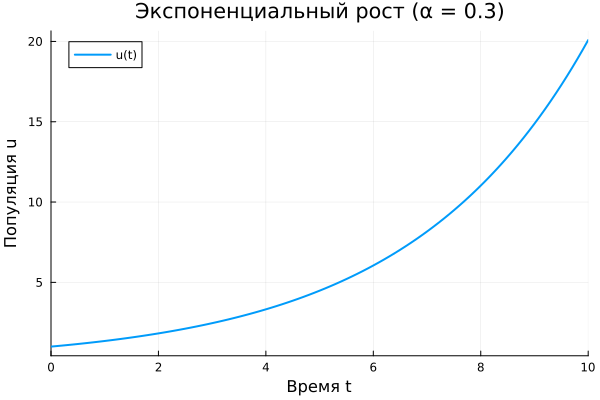
\includegraphics[width=0.68\linewidth,height=\textheight,keepaspectratio]{image/base_growth.png}

\[
u_0=1,\qquad \alpha=0.3,\qquad t\in[0;10].
\]

\textbf{Результат:}\\
\(u(10)\approx20.09\), время удвоения \(T_2\approx2.31\).
\end{frame}

\begin{frame}[fragile]{Организация вычислений}
\protect\phantomsection\label{ux43eux440ux433ux430ux43dux438ux437ux430ux446ux438ux44f-ux432ux44bux447ux438ux441ux43bux435ux43dux438ux439}
Для выполнения работы использовались \textbf{Julia и DrWatson}.

\begin{itemize}
\tightlist
\item
  DifferentialEquations --- решение ОДУ;
\item
  Plots --- построение графиков;
\item
  Literate.jl --- создание \texttt{.jl}, \texttt{.ipynb} и
  \texttt{.qmd};
\item
  Quarto --- оформление отчёта и презентации.
\end{itemize}

Все результаты сохранялись внутри структуры проекта DrWatson.
\end{frame}

\begin{frame}{Параметрическое исследование}
\protect\phantomsection\label{ux43fux430ux440ux430ux43cux435ux442ux440ux438ux447ux435ux441ux43aux43eux435-ux438ux441ux441ux43bux435ux434ux43eux432ux430ux43dux438ux435}
Исследованы значения

\[
\alpha=\{0.1,\;0.3,\;0.5,\;0.8,\;1.0\}.
\]

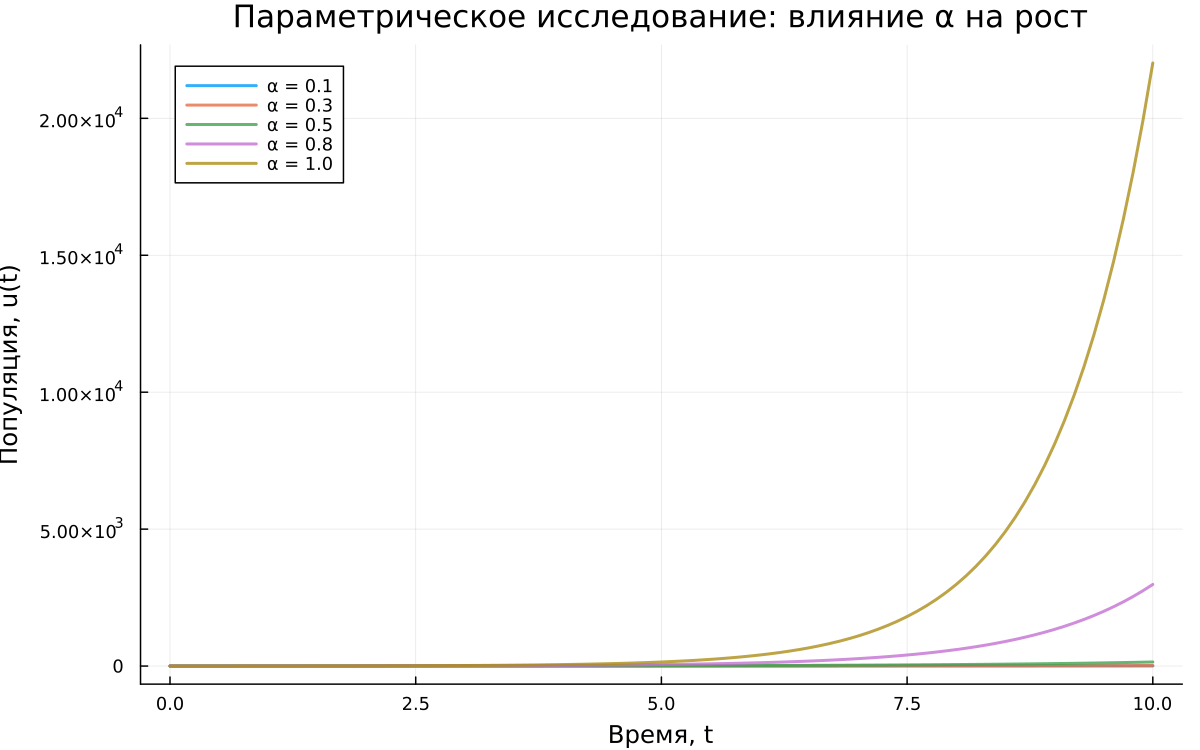
\includegraphics[width=0.78\linewidth,height=\textheight,keepaspectratio]{image/parametric_scan.png}

Чем больше \(\alpha\), тем быстрее растёт функция.
\end{frame}

\begin{frame}{Время удвоения}
\protect\phantomsection\label{ux432ux440ux435ux43cux44f-ux443ux434ux432ux43eux435ux43dux438ux44f}
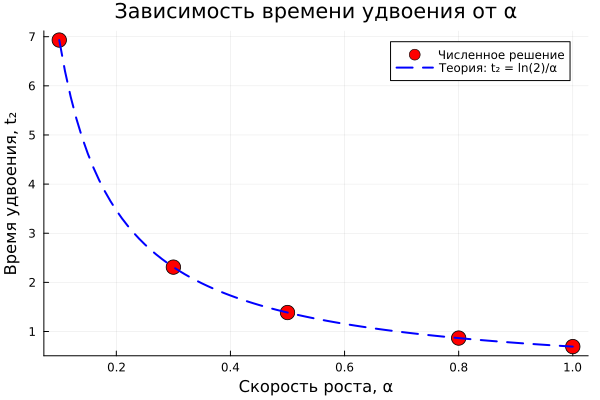
\includegraphics[width=0.72\linewidth,height=\textheight,keepaspectratio]{image/doubling_time.png}

\[
T_2=\frac{\ln2}{\alpha}.
\]

При увеличении \(\alpha\) время удвоения уменьшается.
\end{frame}

\begin{frame}{Численные результаты}
\protect\phantomsection\label{ux447ux438ux441ux43bux435ux43dux43dux44bux435-ux440ux435ux437ux443ux43bux44cux442ux430ux442ux44b}
{\def\LTcaptype{none} % do not increment counter
\begin{longtable}[]{@{}rrr@{}}
\toprule\noalign{}
\(\alpha\) & \(u(10)\) & \(T_2\) \\
\midrule\noalign{}
\endhead
0.1 & 2.72 & 6.93 \\
0.3 & 20.09 & 2.31 \\
0.5 & 148.41 & 1.39 \\
0.8 & 2980.96 & 0.87 \\
1.0 & 22026.47 & 0.69 \\
\bottomrule\noalign{}
\end{longtable}
}

Рост результата с увеличением \(\alpha\) имеет экспоненциальный
характер.
\end{frame}

\begin{frame}{Бенчмаркинг}
\protect\phantomsection\label{ux431ux435ux43dux447ux43cux430ux440ux43aux438ux43dux433}
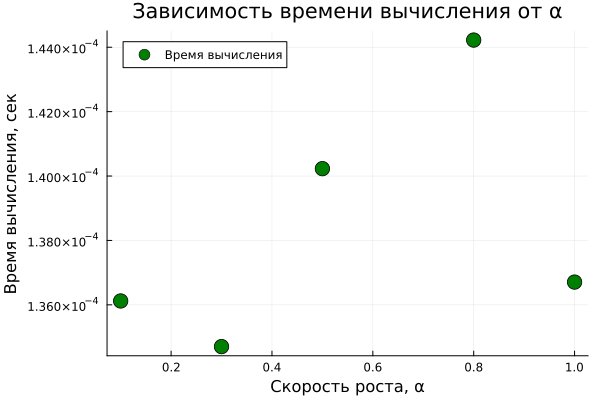
\includegraphics[width=0.67\linewidth,height=\textheight,keepaspectratio]{image/computation_time.png}

Время численного решения для разных значений \(\alpha\) отличается
незначительно.

Различия также зависят от текущей нагрузки компьютера.
\end{frame}

\section{Вывод}\label{ux432ux44bux432ux43eux434}

\begin{frame}{Результаты работы}
\protect\phantomsection\label{ux440ux435ux437ux443ux43bux44cux442ux430ux442ux44b-ux440ux430ux431ux43eux442ux44b}
\begin{itemize}
\tightlist
\item
  реализована модель экспоненциального роста;
\item
  выполнено численное и параметрическое исследование;
\item
  подтверждена зависимость \(T_2=\ln2/\alpha\);
\item
  результаты автоматически сохранены и визуализированы.
\end{itemize}

\textbf{При увеличении \(\alpha\) рост ускоряется, а время удвоения
уменьшается.}
\end{frame}




\end{document}
